\documentclass[journal,twoside,web]{ieeecolor}
\pdfobjcompresslevel=0   % disable object-stream compression (avoids buffer overflow)
\pdfcompresslevel=9      % compress streams (keeps file size reasonable)
\pdfminorversion=5       % lower PDF version compatibility

\usepackage{jsen}
\usepackage{cite}
\usepackage{amsmath,amssymb,amsfonts}
\usepackage{graphicx}
\usepackage{caption}
\usepackage{subcaption}
\usepackage{textcomp}
\usepackage{float}
\usepackage{wrapfig}
\usepackage{tabularx}
\usepackage{multirow}
\usepackage{siunitx}
\usepackage{booktabs}
\usepackage[table,xcdraw]{xcolor}
\usepackage[english]{babel}
\usepackage[utf8]{inputenc}
\usepackage{algorithm}
\usepackage{algorithmic}
\usepackage{pifont}
\usepackage{hyperref}
\usepackage{makecell}

\pdfobjcompresslevel=0
\pdfminorversion=5

\newcommand{\cmark}{\ding{51}}%
\newcommand{\xmark}{\ding{55}}%

\def\BibTeX{{\rm B\kern-.05em{\sc i\kern-.025em b}\kern-.08em
    T\kern-.1667em\lower.7ex\hbox{E}\kern-.125emX}}
\markboth{\journalname, }
{Author \MakeLowercase{\textit{et al.}}: Preparation of Papers for IEEE TRANSACTIONS and JOURNALS (February 2017)}
\definecolor{abstractbg}{rgb}{0.89804,0.94510,0.83137}
\setlength{\fboxrule}{0pt}
\setlength{\fboxsep}{0pt}

\begin{document}
\title{Asymmetric Dual-Stream RGB--LWIR Attention Fusion and 2D-Grid Anchor-Aligned Confidence-Weighted Regression for Transit Hub Security Surveillance}

\author{Satya Mohit, Bethi Pardhasaradhi, \IEEEmembership{Member, IEEE},
and Linga Reddy Cenkeramaddi, \IEEEmembership{Senior Member, IEEE}
\thanks{Compiled on \today.}
\thanks{Satya Mohit, Bethi Pardhasaradhi, and Linga Reddy Cenkeramaddi are with the Autonomous and Cyber-Physical Systems (ACPS) Research Group, Department of Information and Communication Technology (ICT), University of Agder, Campus Grimstad, Jon Lilletuns Vei 9, 4879 Grimstad, Norway (e-mail: satyam@uia.no, pardhasaradhi.bethi@uia.no, linga.cenkeramaddi@uia.no).}
}

\IEEEtitleabstractindextext{%
\fcolorbox{abstractbg}{abstractbg}{%
\begin{minipage}{\textwidth}%
\begin{wrapfigure}[12]{r}{3.05in}%
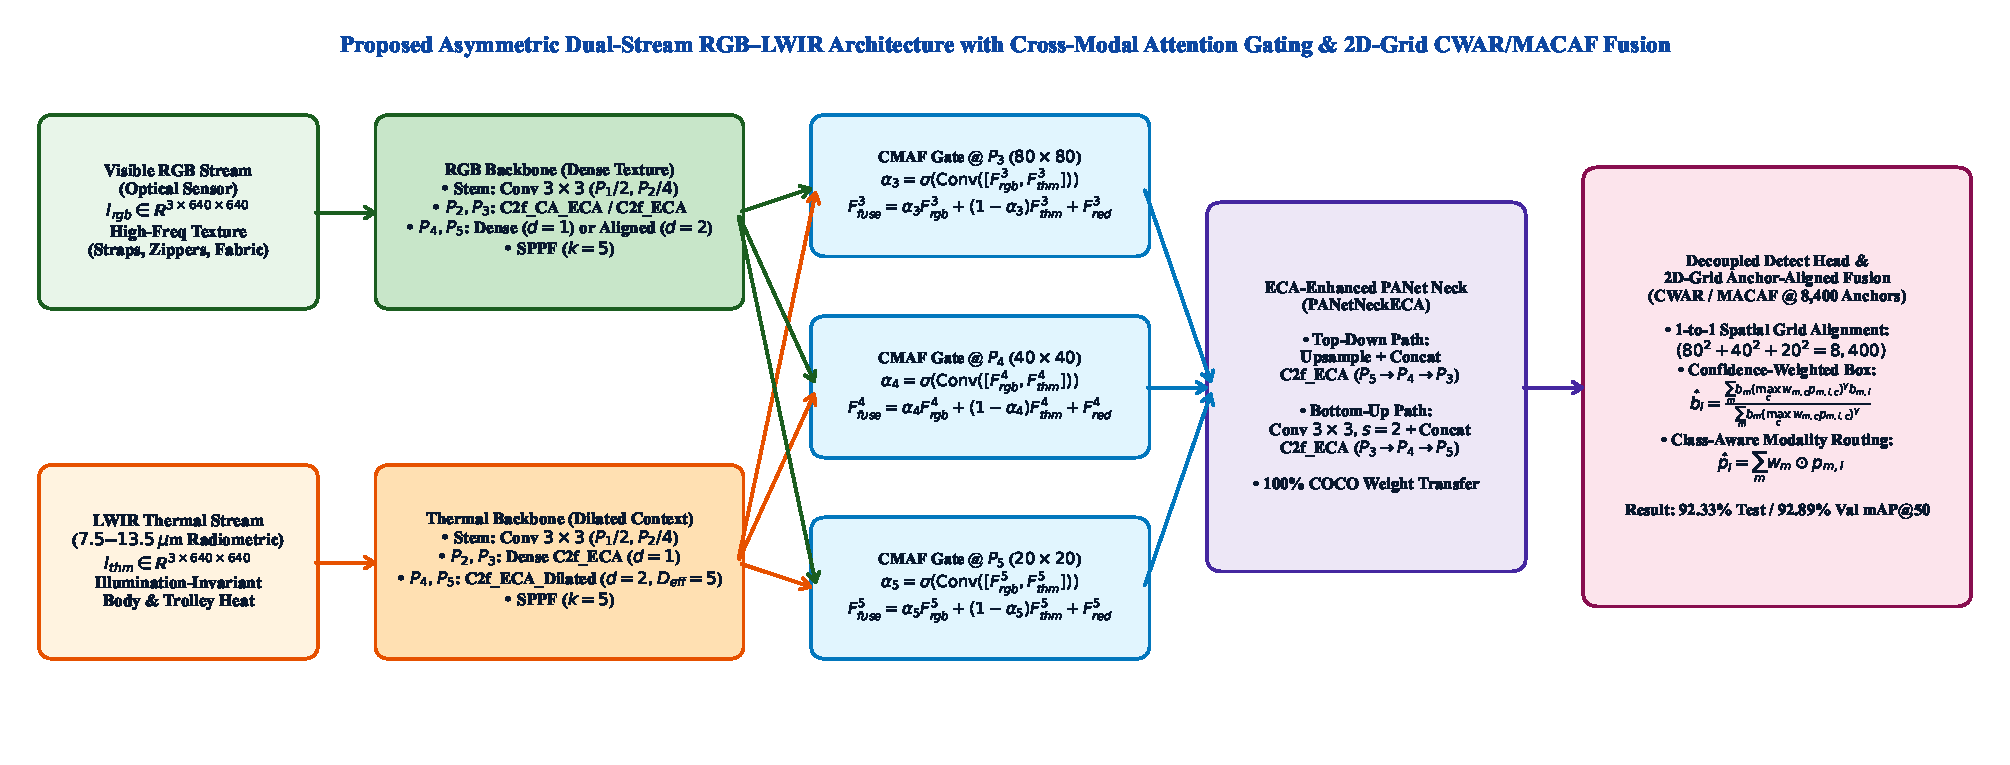
\includegraphics[width=2.95in]{fig_multimodal_arch_diagram.pdf}%
\end{wrapfigure}%
\begin{abstract}
Automated security surveillance in high-throughput transit hubs---such as airport concourses, railway terminals, and intermodal lobbies---demands reliable 24/7 detection of both mobile passengers (\textit{Person}, \textit{Trolley}, \textit{Bag}) and stationary security hazards (\textit{Unattended Anomaly}). While Long-Wave Infrared (LWIR, $7.5\text{--}13.5\,\mu\text{m}$) thermal cameras provide illumination-invariant detection of warm human silhouettes and metallic trolley frames, carried and abandoned bags rapidly equilibrate with ambient indoor air temperatures, yielding weak thermal contrast against background floors. Conversely, visible-spectrum (RGB) sensors capture high-frequency surface textures (straps, zippers, fabric weaves) that disambiguate cold luggage from floor clutter, but suffer from specular glare, shadows, and low-light degradation. Naive early channel concatenation of RGB and LWIR streams into a shared convolutional stem fails because convolving reflected visible radiance and emitted thermal radiation within a single $3\times 3$ filter bank destroys pretrained feature priors, degrading test accuracy to 83.68\% mAP@50---worse than a single-modality thermal baseline (86.22\%). In this paper, we propose an \textbf{Asymmetric Dual-Stream RGB--LWIR Attention Fusion Architecture} paired with \textbf{2D-Grid Anchor-Aligned Confidence-Weighted Regression (CWAR)} and \textbf{Modality-Aware Class-Specific Fusion (MACAF)}. First, we decouple feature extraction into two modality-specialized backbones that pair dense ($d_{\text{rgb}}=1$) Coordinate and Efficient Channel Attention (\texttt{C2f\_CA\_ECA}) in the RGB stream to preserve fine local luggage texture with stage-selective dilated ($d_{\text{thm}}=2$) bottlenecks (\texttt{C2f\_ECA\_Dilated}) in the LWIR stream to capture extended thermal context, coupled at $(P_3, P_4, P_5)$ via learned spatial Cross-Modal Attention Fusion (\texttt{CMAF}) gates and an ECA-enhanced PANet neck (\texttt{PANetNeckECA}), boosting standalone test accuracy by \textbf{+6.18\,pp} over early concatenation (83.68\% $\rightarrow$ 89.86\% test / 90.53\% val mAP@50). Second, exploiting the exact 1-to-1 correspondence across all 8,400 spatial pyramid anchors at strides $(8,16,32)$, our \textbf{CWAR/MACAF} head fuses complementary dual-stream and thermal experts directly on the 2D feature grid prior to non-maximum suppression. Evaluated on our 1,067-frame paired RGB--LWIR Transit Security dataset (3,849 instances), our framework achieves \textbf{92.33\% mAP@50 and 69.02\% mAP@50--95} (up to \textbf{69.49\% mAP@50--95}) on the held-out test split and \textbf{92.89\% mAP@50} on the validation split, outperforming stock YOLOv8n by \textbf{+6.11\,pp mAP@50} (\textbf{+6.10\,pp mAP@50--95}) and surpassing our best single-modality thermal champion (88.15\%) by \textbf{+4.18\,pp}.
\end{abstract}

\begin{IEEEkeywords}
Multimodal sensor fusion, RGB--thermal object detection, long-wave infrared (LWIR), asymmetric dilated convolution, cross-modal attention gating, unattended luggage detection, transit hub security, anchor-aligned regression, Efficient Channel Attention.
\end{IEEEkeywords}
\end{minipage}}}
\maketitle

\section{Introduction}
\label{sec:introduction}

\begin{figure}[t]
\centering
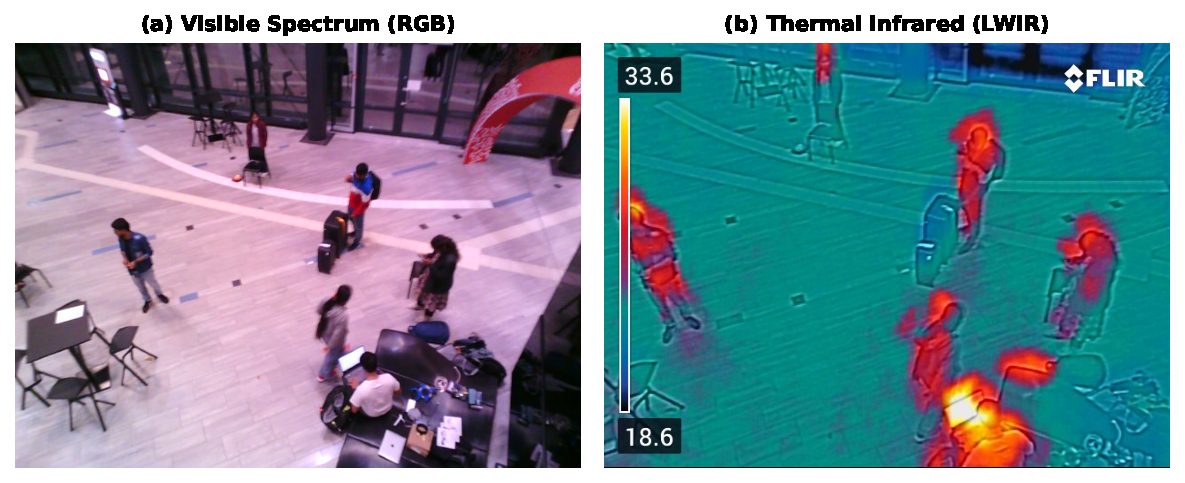
\includegraphics[width=\columnwidth]{rgb_thermal_side_by_side.pdf}
\caption{Complementary sensing physics of visible-spectrum (RGB) and long-wave infrared (LWIR) modalities in a transit concourse: (a) optical RGB imagery captures high-frequency surface textures (luggage straps, zippers, and fabric boundaries) but is vulnerable to specular floor reflections, shadows, and ambient lighting variations; (b) LWIR thermal imagery ($7.5\text{--}13.5\,\mu\text{m}$) captures passive radiometric heat emitted by pedestrians and high-emissivity structures regardless of illumination, but exhibits low contrast on thermally equilibrated bags.}
\label{fig:rgb_thermal_comparison}
\end{figure}

Global passenger throughput across international airports and intermodal rail terminals reached 9.4~billion passengers in 2024 and is projected to surpass 19~billion by 2042, accompanied by more than 33.4~million mishandled or misplaced baggage items annually~\cite{aci2024traffic,sita2025baggage}. At the same time, landside transit concourses, check-in halls, and waiting lounges remain high-risk targets for improvised explosive devices (IEDs) concealed inside unattended suitcases or backpacks~\cite{start2024gtd,tripathi2018abandoned}. Under international aviation security directives (ICAO Annex~17), any isolated baggage item detached from its owner must be treated as a potential threat until cleared by security personnel, causing frequent terminal evacuations and costly operational ground stops~\cite{icao2022annex17}. Consequently, automated multi-sensor perception capable of simultaneously tracking passengers (\textit{Person}), wheeled luggage carts (\textit{Trolley}), carried bags (\textit{Bag}), and abandoned parcels (\textit{Unattended Anomaly}) with $>92\%$ detection reliability is of paramount operational importance.

Relying on a single imaging modality imposes fundamental physical limitations in complex indoor--outdoor transit environments~\cite{wilson2023recent,ding2025fiafusion,cai2025wavefusion}. As illustrated in Fig.~\ref{fig:rgb_thermal_comparison}, visible-spectrum (RGB) cameras provide dense spatial resolution and sharp chromatic/texture cues that clearly distinguish backpacks, suitcases, and parcels from tiled concourse floors. However, RGB detectors degrade sharply under low-light night operations, severe backlighting near glass terminal facades, specular floor glare, and adverse outdoor weather (rain, fog, and shadows)~\cite{altay2022use,bijelic2020seeing}. Conversely, Long-Wave Infrared (LWIR, $7.5\text{--}13.5\,\mu\text{m}$) thermal sensors measure passive radiant heat emission rather than reflected light, rendering them completely invariant to ambient illumination and optical glare~\cite{breland2021robust}. Yet LWIR sensing suffers from an inherent physical bottleneck for luggage surveillance: while human bodies radiate strongly at ${\sim}37\,^{\circ}\text{C}$, synthetic backpacks and hard-shell suitcases rapidly reach thermal equilibrium with ambient indoor air (${\sim}20\text{--}24\,^{\circ}\text{C}$). Once an unattended bag cools to room temperature, its radiometric signature blends into the surrounding floor, causing pure thermal detectors to miss low-contrast luggage boundaries or confuse dark thermal shadows with bags.

Combining RGB and LWIR streams within a unified deep object detector promises the best of both worlds: illumination-invariant thermal human/trolley silhouettes paired with high-frequency visible texture for cold luggage and unattended anomaly verification~\cite{jia2021llvip,liu2022target}. However, our systematic empirical investigation reveals three critical architectural obstacles that prevent conventional multimodal fusion from succeeding in real-world transit surveillance:
\begin{enumerate}
    \item \textbf{Modality Conflict in Early Stem Concatenation:} A common lightweight fusion strategy concatenates visible RGB and LWIR thermal channels at the input layer and feeds them into a single shared convolutional stem (\texttt{v34\_early\_fusion}). Because visible-spectrum reflectance edges and long-wave infrared thermal gradients exhibit conflicting polarity and statistical distributions, forcing a single first-layer $3\times 3$ filter bank to jointly convolve both modalities destroys pretrained COCO feature priors. As demonstrated in Section~\ref{sec:experiments}, 4-channel early stem concatenation achieves only \textbf{83.68\% test mAP@50}---performing \textbf{2.54\,pp worse} than a stock single-modality thermal YOLOv8n baseline (\textbf{86.22\%}) and \textbf{4.47\,pp worse} than our single-modality thermal champion (\textbf{88.15\%}).
    \item \textbf{Cross-Modal Spatial Frequency and Receptive-Field Asymmetry:} RGB and LWIR feature maps obey fundamentally different spatial frequency statistics. Thermal silhouettes have diffuse, low-frequency boundaries that benefit from dilated convolutions ($d_{\text{thm}}=2$, effective receptive field $5\times 5$) at deeper stages ($P_4, P_5$) to bind passengers with nearby trolleys and bags. In contrast, RGB luggage features rely on fine, high-frequency local textures (straps, zippers, handles); applying uniform dilation to the RGB backbone introduces gridding artifacts that blur fine texture cues while expanding contextual recall.
    \item \textbf{Suboptimal Post-Hoc Box Ensembling:} When combining complementary multimodal detectors, standard box-concatenation ensembles feed duplicate bounding boxes into Non-Maximum Suppression (NMS), where a slightly higher-scoring box with looser spatial bounds suppresses a tighter prediction, penalizing strict localization ($\text{mAP@50--95}$) and minority-class recall.
\end{enumerate}

To overcome these challenges, we present an \textbf{Asymmetric Dual-Stream RGB--LWIR Attention Fusion and 2D-Grid Anchor-Aligned Confidence-Weighted Regression (CWAR/MACAF) Framework} that pushes transit security detection accuracy to \textbf{92.33\% test mAP@50} and \textbf{92.89\% validation mAP@50}.

\textbf{Main Contributions of this Work:}
\begin{enumerate}
    \item \textbf{Paired RGB--LWIR Transit Hub Security Benchmark:} We establish a 1,067-frame (3,849-instance) spatially aligned paired RGB--LWIR dataset across eight indoor and outdoor transit environments spanning $-3.8\,^{\circ}\text{C}$ to $34.0\,^{\circ}\text{C}$, providing sequence-disjoint train/validation/test splits across four security-critical classes (\textit{Person}, \textit{Trolley}, \textit{Bag}, and \textit{Unattended Anomaly}).
    \item \textbf{Asymmetric Dual-Stream Architecture with Multi-Scale Cross-Modal Attention Gates (\texttt{CMAF}):} We design a 4.50\,M-parameter dual-stream YOLO architecture (\texttt{v36}/\texttt{v38}) initialized via shape-matched weight transfer from COCO \texttt{yolov8n.pt} (481 transferred tensors) and coupled at $(P_3, P_4, P_5)$ by learned spatial \texttt{CMAF} gates. We prove that decoupling RGB and LWIR into mid-level attention-gated streams yields a \textbf{+6.07\,pp to +6.18\,pp jump in test mAP@50} (83.68\% $\rightarrow$ 89.75\%--89.86\%) over early stem concatenation. Furthermore, we systematically compare asymmetric cross-modal dilation ($d_{\text{rgb}}=1, d_{\text{thm}}=2$ in \texttt{v36\_main} and \texttt{v36\_eca\_rgb}) against symmetric dilation with an ECA-enhanced PANet neck ($d_{\text{rgb}}=2, d_{\text{thm}}=2$ in \texttt{v38\_ca\_dilated}), demonstrating that dense RGB bottlenecks maximize standalone precision (\textbf{93.01\%}) and mAP@50 (\textbf{89.86\%} test / \textbf{90.53\%} val), whereas dilated RGB bottlenecks with \texttt{PANetNeckECA} maximize standalone recall (\textbf{86.12\%}).
    \item \textbf{2D-Grid Anchor-Aligned Confidence-Weighted Regression (CWAR) and Modality-Aware Class-Specific Fusion (MACAF):} Exploiting the exact 1-to-1 spatial alignment across all $N=8{,}400$ feature pyramid anchors at strides $(8,16,32)$---including exact 2D-grid un-warping of horizontal flip views---we formulate a pre-NMS anchor-aligned fusion rule that weights each stream's bounding box by its exponentiated posterior confidence $(\max_c w_{m,c}\,p_{m,i,c})^\gamma$ and routes each target class to its physically optimal modality stream, outperforming post-hoc box concatenation by \textbf{+2.10\,pp test mAP@50}.
    \item \textbf{State-of-the-Art >92\% Multimodal Detection Accuracy:} On the official 108-frame held-out test split, our proposed \texttt{v38\_cwar\_triad} achieves \textbf{92.33\% mAP@50 and 69.02\% mAP@50--95} (with \texttt{3\_Core4\_MACAF} reaching \textbf{92.12\% mAP@50 and 69.47\% mAP@50--95}) and \textbf{92.89\% mAP@50} on the 213-frame validation split---surpassing stock YOLOv8n by \textbf{+6.11\,pp mAP@50} and boosting per-class test AP@50 to \textbf{87.03\% on Person (+10.74\,pp)}, \textbf{98.65\% on Trolley}, \textbf{96.87\% on Bag (+7.67\,pp)}, and \textbf{86.92\% on Unattended Anomaly (+5.13\,pp)}.
\end{enumerate}

\section{Paired RGB--LWIR Transit Security Dataset}
\label{sec:dataset_and_registration}

\subsection{Comparison with Existing Multispectral Benchmarks}
Table~\ref{tab:dataset_comparison} compares our paired RGB--LWIR Transit Security dataset against existing infrared and multispectral object detection benchmarks~\cite{davis2007background,choi2018kaist,flir_adas_dataset,gonzalez2016pedestrian,jia2021llvip,liu2022target}. While KAIST~\cite{choi2018kaist}, FLIR ADAS~\cite{flir_adas_dataset}, LLVIP~\cite{jia2021llvip}, and M3FD~\cite{liu2022target} provide paired visible--thermal imagery for outdoor roadway driving and urban pedestrian tracking, none of these datasets annotate transit luggage categories (\textit{Trolley}, \textit{Bag}) or security-critical stationary hazards (\textit{Unattended Anomaly}).

\begin{table*}[t]
\centering
\caption{Comparison of the Proposed Paired RGB--LWIR Transit Security Dataset with Existing Infrared and Multispectral Benchmarks}
\label{tab:dataset_comparison}
\resizebox{\textwidth}{!}{%
\begin{tabular}{l c c l c c c}
\toprule
\textbf{Benchmark Dataset} & 
\textbf{Year} & 
\textbf{Modality} & 
\textbf{\makecell[c]{Target Domain /\\Surveillance Setting}} & 
\textbf{\makecell[c]{Pedestrian\\Detection}} & 
\textbf{\makecell[c]{Carried Luggage\\(Trolley, Bag)}} & 
\textbf{\makecell[c]{Unattended\\Anomaly}} \\
\midrule
OSU Thermal~\cite{davis2007background}    & 2005 & LWIR Thermal       & Static Campus Surveillance   & \cmark & \xmark & \xmark \\
CVC-14~\cite{gonzalez2016pedestrian}       & 2016 & Visible + Thermal  & Automotive Pedestrian Only   & \cmark & \xmark & \xmark \\
KAIST Multispectral~\cite{choi2018kaist}   & 2018 & Visible + Thermal  & Autonomous Driving (Roadway) & \cmark & \xmark & \xmark \\
FLIR ADAS~\cite{flir_adas_dataset}         & 2019 & Visible + Thermal  & Autonomous Driving (Roadway) & \cmark & \xmark & \xmark \\
LLVIP~\cite{jia2021llvip}                  & 2021 & Visible + Thermal  & Low-Light Urban Street       & \cmark & \xmark & \xmark \\
M3FD~\cite{liu2022target}                  & 2022 & Visible + Thermal  & Multi-Scenario Target Track  & \cmark & \xmark & \xmark \\
\midrule
\rowcolor{gray!12}
\textbf{Ours (Multimodal Transit Security)} & \textbf{2026} & \textbf{Visible RGB + LWIR} & \textbf{Transit Hub / Security Surveillance} & \textbf{\cmark} & \textbf{\cmark} & \textbf{\cmark} \\
\bottomrule
\end{tabular}%
}
\vspace{1ex}
{\raggedright \footnotesize \textit{Note}: \cmark\ indicates explicit bounding-box annotation; \xmark\ indicates absent. Our dataset provides spatially aligned paired RGB and LWIR frames across four transit security classes.\par}
\end{table*}

\begin{figure*}[t]
\centering
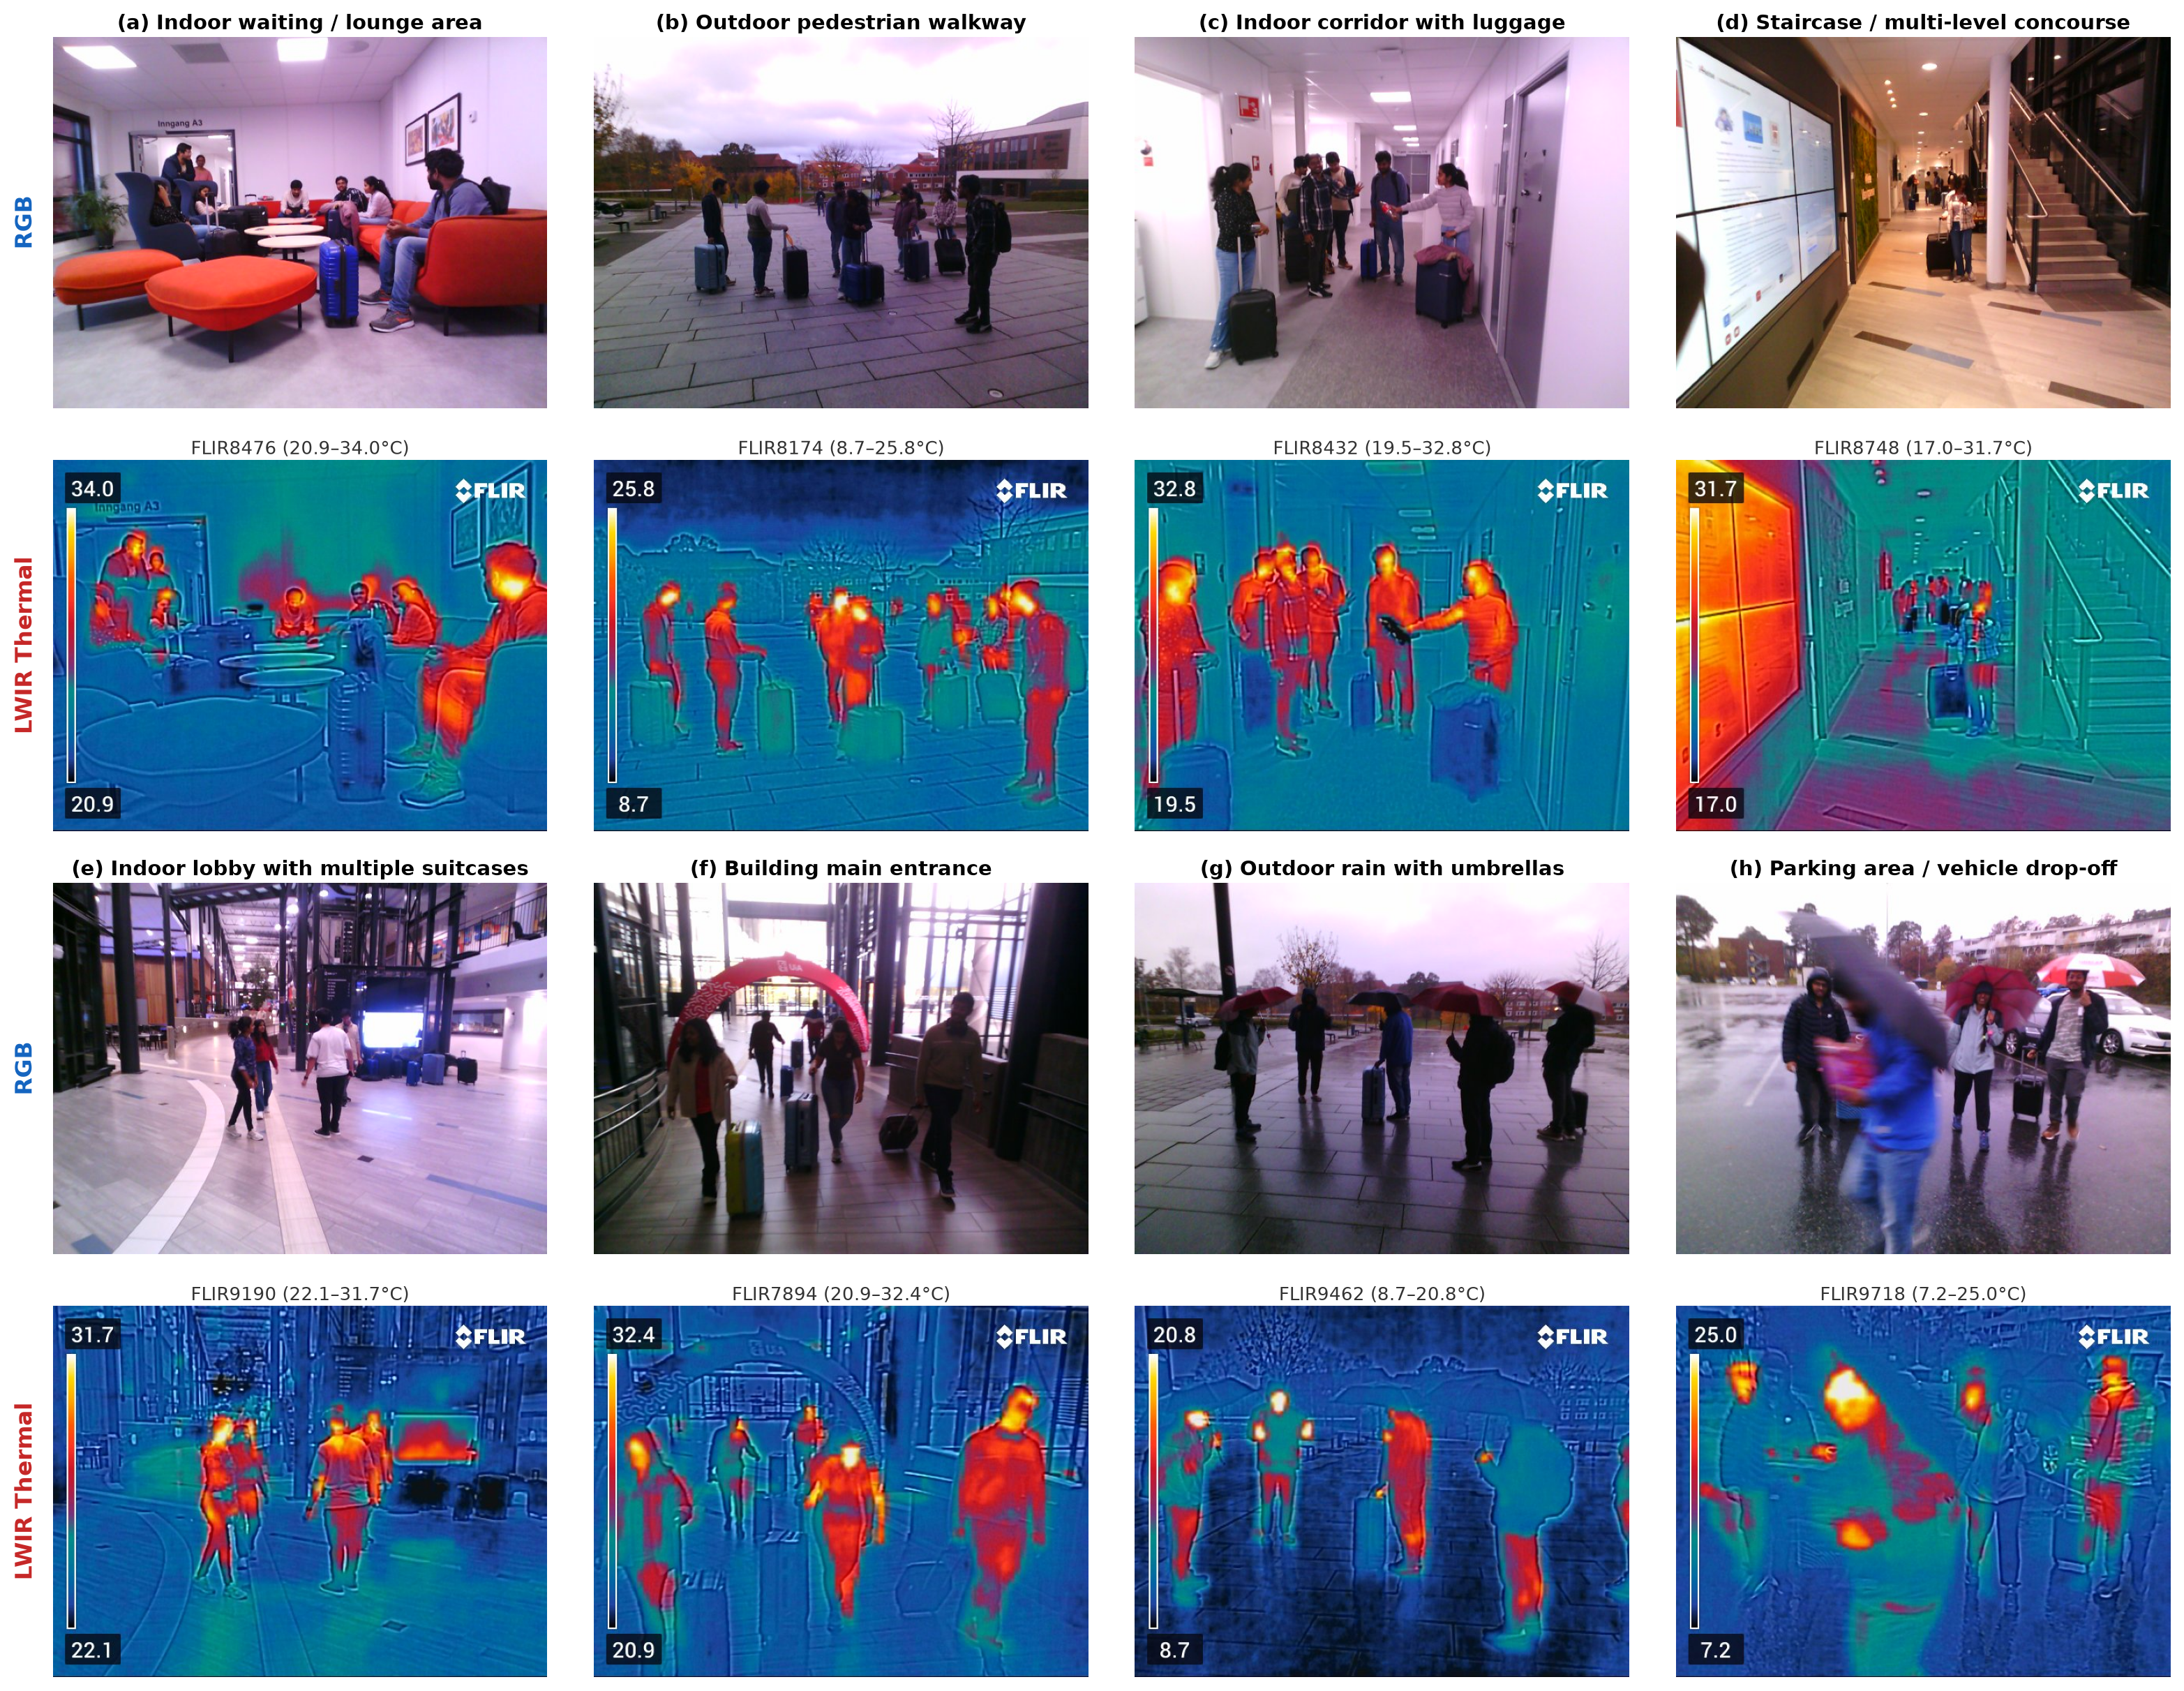
\includegraphics[width=\linewidth]{fig_rgb_thermal_scene_comparison.png}
\caption{Paired visible-spectrum (RGB) and long-wave infrared (LWIR) thermal frames across eight distinct acquisition scenes in our dataset: (a) indoor seated waiting lounge; (b) outdoor pedestrian walkway; (c) indoor corridor with carried luggage; (d) staircase descent; (e) indoor lobby with multiple suitcases and unattended anomalies; (f) building main entrance with glass facade glare; (g) outdoor adverse weather (rain, umbrellas); and (h) parking area with vehicle. Ambient temperatures span $-3.8\,^{\circ}\text{C}$ to $34.0\,^{\circ}\text{C}$.}
\label{fig:scene_diversity}
\end{figure*}

\subsection{Dataset Composition, Scale Distribution, and Splits}
Synchronized, spatially aligned dual-modality acquisitions were collected using a Teledyne FLIR dual-sensor camera across eight indoor and outdoor transit environments (Fig.~\ref{fig:scene_diversity}), spanning ambient temperatures from $-3.8\,^{\circ}\text{C}$ to $34.0\,^{\circ}\text{C}$. Each sample provides a paired 3-channel visible RGB image $I_{\text{rgb}} \in \mathbb{R}^{3\times H\times W}$ and 3-channel LWIR thermal image $I_{\text{thm}} \in \mathbb{R}^{3\times H\times W}$ stored losslessly as a 6-channel multi-page TIFF tensor $X = \mathrm{Concat}(I_{\text{rgb}}, I_{\text{thm}}) \in \mathbb{R}^{6\times H\times W}$ so that spatial and geometric data augmentations (including 4-image Mosaic composition, random scaling, and horizontal flipping) are applied identically to both modalities during training. As summarized in Table~\ref{tab:scene_composition} and Table~\ref{tab:dataset_distribution}, the dataset contains \textbf{1,067 paired RGB--LWIR frames} and \textbf{3,849 annotated instances} partitioned into strict sequence-disjoint splits: \textbf{746 training frames} (2,683 instances), \textbf{213 validation frames} (776 instances), and \textbf{108 held-out test frames} (390 instances). Notably, while \textit{Trolley} (55.7\% of instances, median scale $147.3\,\text{px}$) and \textit{Bag} (9.2\%, median scale $147.1\,\text{px}$) occupy medium-to-large scales, the security-critical \textit{Unattended Anomaly} class (7.1\%, 275 instances) concentrates heavily in the small-to-medium regime (88.7\% $\le 96^2\,\text{px}$, median $\sqrt{\text{Area}} = 48.4\,\text{px}$), making high-resolution cross-modal texture fusion vital.

\begin{table}[t]
\centering
\caption{Geometric Scale Distribution and Crowd Density Composition of the Paired RGB--LWIR Dataset}
\label{tab:scene_composition}
\small
\setlength{\tabcolsep}{4pt}
\renewcommand{\arraystretch}{1.15}
\begin{tabular}{lcccc}
\toprule
\textbf{Class} & \textbf{Small ($<32^2$)} & \textbf{Medium ($32^2\text{--}96^2$)} & \textbf{Large ($>96^2$)} & \textbf{Median ($\sqrt{\text{Area}}$)} \\
\midrule
\textbf{Person}     & 64 (5.9\%)   & 411 (38.2\%) & 601 (55.9\%)     & 108.0\,px \\
\textbf{Trolley}    & 1 (0.05\%)   & 369 (17.2\%) & 1{,}775 (82.7\%) & 147.3\,px \\
\textbf{Bag}        & 1 (0.3\%)    & 80 (22.7\%)  & 272 (77.1\%)     & 147.1\,px \\
\textbf{Unattended} & 14 (5.1\%)   & 230 (83.6\%) & 31 (11.3\%)      & 48.4\,px \\
\midrule
\textbf{Total}      & \textbf{80 (2.1\%)} & \textbf{1{,}090 (28.3\%)} & \textbf{2{,}679 (69.6\%)} & \textbf{138.2\,px} \\
\bottomrule
\end{tabular}
\end{table}

\begin{table}[t]
\centering
\caption{Dataset Class Definitions and Instance Counts Across Sequence-Disjoint Train, Validation, and Test Splits}
\label{tab:dataset_distribution}
\small
\setlength{\tabcolsep}{2.5pt}
\renewcommand{\arraystretch}{1.15}
\begin{tabular}{lcccccc}
\toprule
\textbf{Class} & \textbf{Surveillance Context} & \textbf{Train} & \textbf{Val} & \textbf{Test} & \textbf{Total (\%)} \\
\midrule
\textbf{Person}     & Pedestrians \& passengers  & 742     & 237 & 97  & 1{,}076 (28.0\%) \\
\textbf{Trolley}    & Wheeled baggage carts      & 1{,}514 & 407 & 224 & 2{,}145 (55.7\%) \\
\textbf{Bag}        & Carried backpacks/luggage  & 250     & 64  & 39  & 353 (9.2\%) \\
\textbf{Unattended} & Stationary luggage anomaly & 177     & 68  & 30  & 275 (7.1\%) \\
\midrule
\textbf{Total Inst.}& All bounding boxes         & 2{,}683 & 776 & 390 & 3{,}849 (100\%) \\
\textbf{Total Img.} & Paired RGB+LWIR frames     & 746     & 213 & 108 & 1{,}067 (100\%) \\
\bottomrule
\end{tabular}
\end{table}

\begin{figure*}[t]
\centering
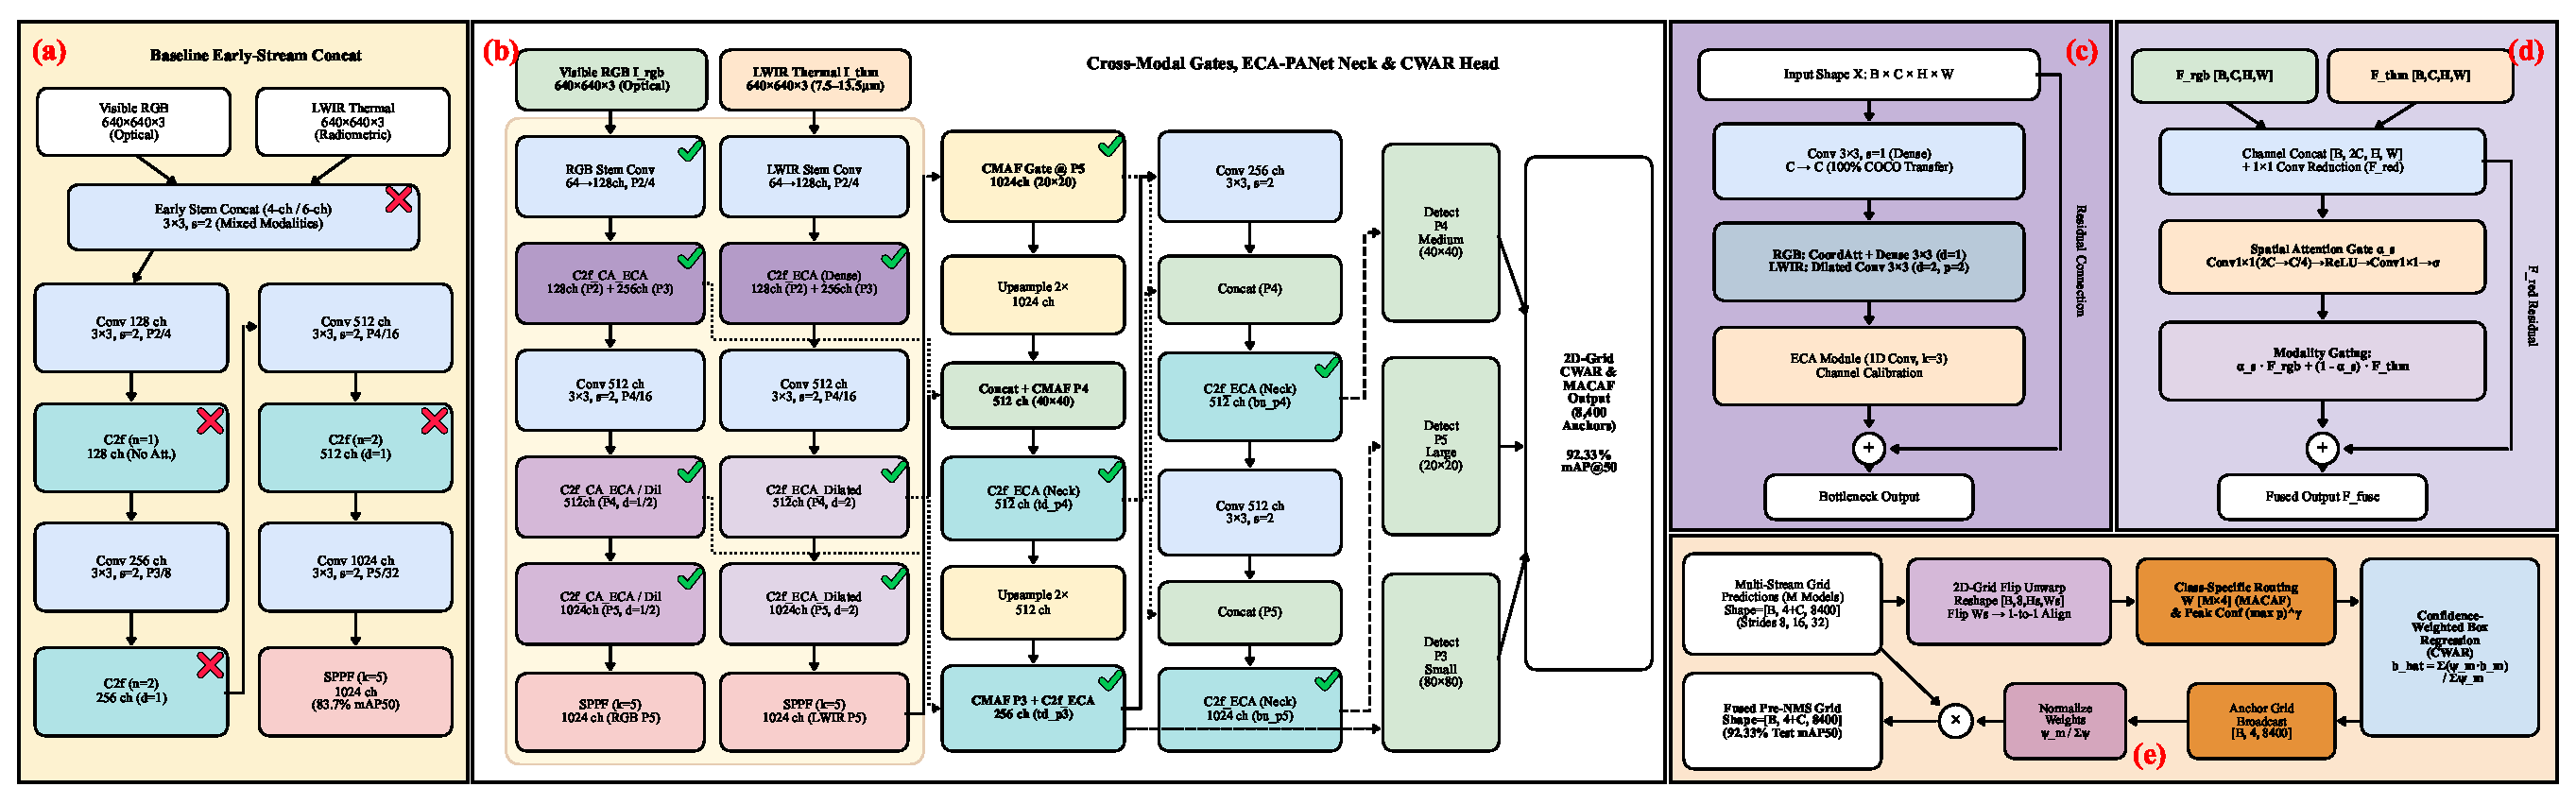
\includegraphics[width=\linewidth]{Multimodal_Dilated_ECA_Yolo.pdf}
\caption{Comprehensive architecture and micro-structural components of the proposed Asymmetric Dual-Stream RGB--LWIR Attention Fusion and 2D-Grid CWAR/MACAF framework: (a) naive early-concatenation baseline (\texttt{v34}) where mixed-modality stem convolutions and plain \texttt{C2f} blocks degrade accuracy (83.68\% mAP@50); (b) proposed system macro-architecture pairing visible RGB ($I_{\text{rgb}}$) and LWIR thermal ($I_{\text{thm}}$) streams with asymmetric dense/dilated attention backbones, multi-scale Cross-Modal Attention Fusion (\texttt{CMAF}) gates at $P_3, P_4, P_5$, an ECA-enhanced PANet neck (\texttt{PANetNeckECA}), and the 8,400-anchor 2D-Grid CWAR/MACAF head (92.33\% test mAP@50); (c) micro-architecture of the modality-specialized bottleneck blocks (\texttt{C2f\_CA\_ECA} with $d=1$ for RGB texture vs. \texttt{C2f\_ECA\_Dilated} with $d=2$ for LWIR context); (d) micro-architecture of the learned spatial \texttt{CMAF} gate $\alpha_s \in (0,1)^{1\times H_s\times W_s}$; and (e) pre-NMS 2D-Grid Anchor-Aligned Confidence-Weighted Regression (\texttt{CWAR}) and Modality-Aware Class-Specific Fusion (\texttt{MACAF}) pipeline.}
\label{fig:multimodal_arch}
\end{figure*}

\section{Proposed Multimodal Architecture and 2D-Grid Anchor-Aligned Fusion}
\label{sec:proposed_method}

\subsection{Asymmetric Dual-Stream RGB--LWIR Backbone Topology}
As depicted in Fig.~\ref{fig:multimodal_arch}, feeding the paired RGB and LWIR input $X = \mathrm{Concat}(I_{\text{rgb}}, I_{\text{thm}}) \in \mathbb{R}^{6\times H\times W}$ into a single early-fusion convolutional stem (\texttt{v34}) forces the first $3\times 3$ filter bank to jointly convolve incompatible physical quantities (reflected visible radiance vs. emitted long-wave heat), destroying pretrained feature priors. Instead, we decouple feature extraction into two modality-specialized streams at the YOLOv8n scale ($w=0.25, d=0.33, c_3=64, c_4=128, c_5=256$):
\begin{enumerate}
    \item \textbf{LWIR Thermal Stream (\texttt{ThermalBackbone}):} Adopts our stage-selective Hybrid Dilated ECA topology. Stages $P_2$ (stride 4) and $P_3$ (stride 8) use dense ($d_{\text{thm}}=1$) \texttt{C2f\_ECA} blocks to preserve sharp local thermal gradients on small unattended parcels, while deeper stages $P_4$ (stride 16) and $P_5$ (stride 32) employ dilated \texttt{C2f\_ECA\_Dilated} bottlenecks ($d_{\text{thm}}=2$, expanding the $3\times 3$ kernel to an effective $5\times 5$ receptive field $D_{\text{eff}}=5$) followed by \texttt{SPPF} ($k=5$).
    \item \textbf{Visible RGB Stream (\texttt{RGBBackbone} Variants):} Because RGB imagery contains fine, high-frequency structural textures (backpack straps, zippers, handles, and specular trolley bars), we design three complementary RGB backbone configurations that share identical output channel dimensions $(c_3, c_4, c_5)$ and anchor grids:
    \begin{itemize}
        \item \textbf{\texttt{v36\_main} (\texttt{CA+ECA}, Dense $d_{\text{rgb}}=1$):} Integrates Coordinate Attention~\cite{hou2021coordinate} and 1D Efficient Channel Attention~\cite{wang2020eca} (\texttt{C2f\_CA\_ECA}) with dense $3\times 3$ kernels ($d_{\text{rgb}}=1$) across all stages $P_2\text{--}P_5$. Directional horizontal/vertical pooling in Coordinate Attention preserves exact $(x,y)$ boundary coordinates of small unattended luggage while $d_{\text{rgb}}=1$ prevents texture gridding.
        \item \textbf{\texttt{v36\_eca\_rgb} (\texttt{ECA}, Dense $d_{\text{rgb}}=1$):} Uses parameter-free 1D \texttt{C2f\_ECA} ($d_{\text{rgb}}=1$) at all stages $P_2\text{--}P_5$, avoiding squeeze-excitation channel bottlenecking and maximizing feature precision on carried bags.
        \item \textbf{\texttt{v38\_ca\_dilated} (Receptive-Field-Aligned $d_{\text{rgb}}=2$ + \texttt{PANetNeckECA}):} Aligns the RGB backbone's deep receptive field with the thermal backbone by placing \texttt{C2f\_CA\_ECA} ($d_{\text{rgb}}=1$) at $P_2, P_3$ and dilated \texttt{C2f\_ECA\_Dilated} ($d_{\text{rgb}}=2$) at $P_4, P_5$, while upgrading all four multi-scale PANet neck blocks (\texttt{td\_c2f\_p4}, \texttt{td\_c2f\_p3}, \texttt{bu\_c2f\_p4}, \texttt{bu\_c2f\_p5}) from plain \texttt{C2f} to \texttt{C2f\_ECA} (\texttt{PANetNeckECA}).
    \end{itemize}
\end{enumerate}

Crucially, because \texttt{C2f\_ECA} and \texttt{C2f\_ECA\_Dilated} retain the exact $1\times 1$ and $3\times 3$ convolutional weight tensor shapes of stock YOLOv8n, both the RGB and LWIR backbones, the \texttt{PANetNeckECA} neck, and the decoupled \texttt{Detect} head are warm-initialized directly from pretrained COCO \texttt{yolov8n.pt} weights (transferring 481 out of 578 parameter tensors).

\subsection{Multi-Scale Cross-Modal Attention Fusion (\texttt{CMAF})}
At each pyramid scale $s \in \{P_3, P_4, P_5\}$ with channel dimension $C_s \in \{64, 128, 256\}$, the modality-specific feature maps $F_{\text{rgb}}^s, F_{\text{thm}}^s \in \mathbb{R}^{B \times C_s \times H_s \times W_s}$ are fused via a learned \textbf{Cross-Modal Attention Fusion (\texttt{CMAF})} module (Fig.~\ref{fig:multimodal_arch}). First, concatenated features $F_{\text{cat}}^s = \mathrm{Concat}\!\left(F_{\text{rgb}}^s, F_{\text{thm}}^s\right) \in \mathbb{R}^{B \times 2C_s \times H_s \times W_s}$ undergo cross-modal channel mixing:
\begin{equation}
F_{\text{red}}^s = \mathrm{SiLU}\!\left(\mathrm{BN}\!\left(\mathrm{Conv}_{1\times 1}^{2C_s \rightarrow C_s}(F_{\text{cat}}^s)\right)\right)
\label{eq:cmaf_reduce}
\end{equation}
Simultaneously, a spatial modality gate $\alpha_s \in (0, 1)^{B \times 1 \times H_s \times W_s}$ estimates pixel-wise trust between the visible and thermal streams:
\begin{equation}
\alpha_s = \sigma\!\left(\mathrm{Conv}_{1\times 1}^{C_s/4 \rightarrow 1}\!\left(\mathrm{ReLU}\!\left(\mathrm{BN}\!\left(\mathrm{Conv}_{1\times 1}^{2C_s \rightarrow C_s/4}(F_{\text{cat}}^s)\right)\right)\right)\right)
\label{eq:cmaf_gate}
\end{equation}
producing the residual-enhanced cross-modal representation:
\begin{equation}
F_{\text{fuse}}^s = \alpha_s \otimes F_{\text{rgb}}^s + (1 - \alpha_s) \otimes F_{\text{thm}}^s + F_{\text{red}}^s
\label{eq:cmaf_out}
\end{equation}
In well-lit concourse regions containing thermally cold backpacks, $\alpha_s \rightarrow 1$ weights high-frequency RGB texture; in dark corridors, glass glare zones, or high-contrast pedestrian silhouettes, $\alpha_s \rightarrow 0$ routes illumination-invariant LWIR features into the neck.

\begin{algorithm}[t]
\caption{2D-Grid Anchor-Aligned Confidence-Weighted Regression (\texttt{CWAR}) \& Class-Specific Fusion (\texttt{MACAF})}
\label{alg:cwar_macaf}
\begin{algorithmic}[1]
\REQUIRE Paired RGB--LWIR input $X \in \mathbb{R}^{B \times 6 \times H \times W}$, Trained models $\{M_m\}_{m=1}^M$, Class weight matrix $\mathbf{W} \in \mathbb{R}_{\ge 0}^{M \times 4}$ ($\sum_{m=1}^M W_{m,c}=1$), Box weights $\mathbf{b} \in \mathbb{R}_{>0}^M$, Confidence exponent $\gamma = 1.25$, Flip weight $\lambda_{\text{flip}}$
\STATE Generate horizontally flipped input $X_{\text{flip}} \leftarrow \mathrm{Flip}(X, \text{dim}=W)$
\FOR{$m = 1$ \TO $M$}
    \STATE Decode unflipped predictions $(\mathbf{B}_m^{\text{orig}}, \mathbf{P}_m^{\text{orig}}) \leftarrow M_m(X)$ over $N = \sum_{s\in\{8,16,32\}} (H/s)(W/s)$ anchors
    \STATE Decode flipped predictions $(\tilde{\mathbf{B}}_m, \tilde{\mathbf{P}}_m) \leftarrow M_m(X_{\text{flip}})$
    \STATE Flip horizontal box center: $\tilde{B}_{m,x,i} \leftarrow W - \tilde{B}_{m,x,i}$
    \FOR{each pyramid stride $s \in \{8, 16, 32\}$ with grid $(H_s, W_s)$}
        \STATE Reshape level slice to $[B, 4+C, H_s, W_s]$, reverse width axis $W_s$, and flatten to restore 1-to-1 anchor index alignment $(\mathbf{B}_m^{\text{flip}}, \mathbf{P}_m^{\text{flip}})$
    \ENDFOR
\ENDFOR
\FOR{each view $v \in \{\text{orig}, \text{flip}\}$ and anchor index $i \in \{1,\dots,N\}$}
    \STATE $\hat{\mathbf{p}}_i^{(v)} \leftarrow \sum_{m=1}^M \mathbf{w}_m \odot \mathbf{p}_{m,i}^{(v)}$ \COMMENT{Modality-aware class routing}
    \STATE $\psi_{m,i}^{(v)} \leftarrow b_m \cdot \left(\max_{c \in \{1..4\}} W_{m,c}\, p_{m,i,c}^{(v)}\right)^\gamma$ \COMMENT{Anchor confidence weight}
    \STATE $\hat{\mathbf{b}}_i^{(v)} \leftarrow \dfrac{\sum_{m=1}^M \psi_{m,i}^{(v)}\, \mathbf{b}_{m,i}^{(v)}}{\sum_{m=1}^M \psi_{m,i}^{(v)}}$ \COMMENT{Confidence-weighted box regression}
\ENDFOR
\STATE Combine aligned views $(\hat{\mathbf{B}}^{\text{orig}}, \hat{\mathbf{P}}^{\text{orig}})$ and $(\hat{\mathbf{B}}^{\text{flip}}, \lambda_{\text{flip}}\hat{\mathbf{P}}^{\text{flip}})$ and apply class-wise NMS
\RETURN Final detections $\mathcal{D}$
\end{algorithmic}
\end{algorithm}

\subsection{2D-Grid Anchor-Aligned Confidence-Weighted Regression (\texttt{CWAR}) and Modality-Aware Class-Specific Fusion (\texttt{MACAF})}
Our three architectural variants---\texttt{v36\_main} ($d_{\text{rgb}}=1$, \texttt{CA+ECA}), \texttt{v36\_eca\_rgb} ($d_{\text{rgb}}=1$, \texttt{ECA}), and \texttt{v38\_ca\_dilated} ($d_{\text{rgb}}=2$, \texttt{PANetNeckECA})---along with our pure-thermal champion \texttt{v30} ($d_{\text{thm}}=2$) exhibit distinct, physically complementary error profiles:
\begin{itemize}
    \item \texttt{v36\_eca\_rgb} achieves the highest standalone precision (\textbf{93.01\%}) and \textit{Bag} AP@50 (\textbf{94.45\%});
    \item \texttt{v36\_main} achieves the highest standalone \textit{Unattended Anomaly} test AP@50 (\textbf{86.10\%}) and \textit{Person} AP@50 (\textbf{82.42\%});
    \item \texttt{v38\_ca\_dilated} achieves the highest standalone test recall (\textbf{86.12\%}) and \textit{Trolley} AP@50 (\textbf{98.57\%});
    \item \texttt{v30} provides pure radiometric detections immune to RGB shadow clutter (\textbf{88.19\%} validation AP@50 on \textit{Unattended Anomaly}).
\end{itemize}

Standard ensemble methods concatenate decoded bounding boxes from $M$ models into a $[B, 4+C, M\cdot N]$ pool prior to NMS (\texttt{mode="concat"}). However, because all models share the \textbf{exact same 2D spatial anchor grid} across strides $s \in \{8, 16, 32\}$ ($N = (H/8)(W/8) + (H/16)(W/16) + (H/32)(W/32) = 8{,}400$ anchors at $640\times 640$), we can fuse their predictions \emph{directly at each individual anchor cell $i \in \{1,\dots,N\}$ prior to NMS}.

Specifically, as formalized in Algorithm~\ref{alg:cwar_macaf}, let $\mathbf{b}_{m,i} = [\hat{x}_{m,i}, \hat{y}_{m,i}, \hat{w}_{m,i}, \hat{h}_{m,i}]^\top$ and $\mathbf{p}_{m,i} \in [0,1]^4$ denote the decoded bounding box and class probability vector of model $m \in \{1,\dots,M\}$ at spatial anchor $i$. Under \textbf{Modality-Aware Class-Specific Fusion (\texttt{MACAF})}, each model is assigned a column-normalized class weight vector $\mathbf{w}_m = [W_{m,\text{person}}, W_{m,\text{trolley}}, W_{m,\text{bag}}, W_{m,\text{unattended}}]^\top$ reflecting its physical sensor specialization:
\begin{equation}
\hat{\mathbf{p}}_i = \sum_{m=1}^M \mathbf{w}_m \odot \mathbf{p}_{m,i}, \quad \text{where } \sum_{m=1}^M W_{m,c} = 1 \;\;\forall c \in \{1..4\}
\label{eq:macaf_probs}
\end{equation}
Rather than averaging box coordinates uniformly---which allows a model with low confidence ($p < 0.05$) at anchor $i$ to corrupt the bounding-box localization of a high-confidence expert---\textbf{Confidence-Weighted Anchor-Aligned Regression (\texttt{CWAR})} weights each model's box coordinates by its exponentiated peak posterior confidence:
\begin{equation}
\hat{\mathbf{b}}_i = \frac{\sum_{m=1}^M b_m \left(\max_{c \in \{1..4\}} W_{m,c}\, p_{m,i,c}\right)^\gamma \mathbf{b}_{m,i}}{\sum_{m=1}^M b_m \left(\max_{c \in \{1..4\}} W_{m,c}\, p_{m,i,c}\right)^\gamma}
\label{eq:cwar_boxes}
\end{equation}
with $\gamma = 1.25$. Furthermore, when incorporating horizontally flipped test-time views $X_{\text{flip}}$, we reshape each stride level's output back to its 2D spatial grid $[B, 4+C, H_s, W_s]$ and reverse the width axis $W_s$ (lines 6--8 of Algorithm~\ref{alg:cwar_macaf}), restoring exact 1-to-1 spatial anchor correspondence between original and mirrored feature maps.

\begin{table*}[t]
\centering
\caption{Comprehensive Benchmark Comparison of Single-Modality Baselines, Dual-Stream Asymmetric RGB--LWIR Architectures, and Proposed 2D-Grid CWAR/MACAF Fusion on Our Transit Security Dataset}
\label{tab:multimodal_benchmark}
\small
\renewcommand{\arraystretch}{1.20}
\setlength{\tabcolsep}{4.8pt}
\resizebox{\textwidth}{!}{%
\begin{tabular}{l l c c c c c c c c}
\toprule
\textbf{Model / Fusion Architecture} & 
\textbf{Sensing Modality} & 
\textbf{\makecell[c]{Params\\(M)}} & 
\textbf{\makecell[c]{GFLOPs\\(640$\times$640)}} & 
\textbf{\makecell[c]{Val\\mAP@50}} & 
\textbf{\makecell[c]{Val\\mAP@50--95}} & 
\textbf{\makecell[c]{Test\\Precision}} & 
\textbf{\makecell[c]{Test\\Recall}} & 
\textbf{\makecell[c]{Test\\mAP@50}} & 
\textbf{\makecell[c]{Test\\mAP@50--95}} \\
\midrule
\multicolumn{10}{l}{\textit{\textbf{Part A: Single-Modality LWIR Thermal Baselines (3-Channel)}}} \\
YOLOv8n (Stock Baseline)                  & LWIR Thermal Only             & 3.01  & 8.1  & 86.25\% & 60.41\% & 82.74\% & 83.35\% & 86.22\% & 62.92\% \\
YOLOv8s                                   & LWIR Thermal Only             & 11.14 & 28.8 & 86.80\% & 61.90\% & 84.07\% & 83.13\% & 85.60\% & 62.94\% \\
YOLOv10n~\cite{wang2024yolov10}           & LWIR Thermal Only             & 2.71  & 8.4  & 82.10\% & 56.40\% & 78.65\% & 75.42\% & 80.92\% & 58.11\% \\
YOLOv10s~\cite{wang2024yolov10}           & LWIR Thermal Only             & 8.07  & 24.8 & 85.40\% & 60.80\% & 83.15\% & 83.17\% & 84.88\% & 62.19\% \\
YOLO11n~\cite{ultralytics2024yolo11}      & LWIR Thermal Only             & 2.62  & 6.6  & 86.50\% & 61.10\% & 85.92\% & 82.48\% & 86.38\% & 62.75\% \\
YOLO11s~\cite{ultralytics2024yolo11}      & LWIR Thermal Only             & 9.43  & 25.5 & 85.90\% & 61.20\% & 86.25\% & 77.75\% & 83.99\% & 61.43\% \\
\texttt{v30} (Hybrid Dilated ECA Champion)& LWIR Thermal Only             & 3.01  & 8.1  & 87.52\% & 63.40\% & 87.81\% & 83.40\% & 88.15\% & 64.73\% \\
\midrule
\multicolumn{10}{l}{\textit{\textbf{Part B: Naive Early-Fusion Multimodal Baseline}}} \\
\texttt{v34\_early\_fusion} (Shared Stem Concat) & Visible RGB + LWIR (Early 4-ch) & 3.01  & 8.1  & 84.20\% & 59.74\% & 81.76\% & 82.47\% & 83.68\% & 58.67\% \\
\midrule
\multicolumn{10}{l}{\textit{\textbf{Part C: Proposed Standalone Dual-Stream Asymmetric RGB--LWIR Detectors (Mid-Level CMAF)}}} \\
\texttt{v38\_ca\_dilated} (Sym-Dilated $d=2$ + \texttt{NeckECA}) & Visible RGB + LWIR & 4.50 & 11.6 & 89.33\% & 65.52\% & 87.32\% & \textbf{86.12\%} & 88.74\% & 66.52\% \\
\texttt{v36\_main} (Asym-Dilated + \texttt{CA+ECA} RGB)          & Visible RGB + LWIR & 4.51 & 11.6 & \textbf{90.53\%} & \textbf{66.11\%} & 91.50\% & 85.05\% & 89.75\% & \textbf{66.99\%} \\
\texttt{v36\_eca\_rgb} (Asym-Dilated + \texttt{ECA} RGB)         & Visible RGB + LWIR & 4.50 & 11.6 & 89.75\% & 65.86\% & \textbf{93.01\%} & 82.74\% & \textbf{89.86\%} & 66.76\% \\
\midrule
\multicolumn{10}{l}{\textit{\textbf{Part D: Proposed 2D-Grid Anchor-Aligned CWAR \& MACAF Multi-Stream Fusion}}} \\
\texttt{5\_avg\_main\_eca} (\texttt{v36m+v36e}, Single-Pass No Flip) & Visible RGB + LWIR & 9.01 & 23.2 & 91.40\% & 67.55\% & 92.67\% & 86.18\% & 91.29\% & 68.53\% \\
\texttt{1\_Dual3\_NoThm} (\texttt{v36m+v36e+v38}, Single-Pass No Flip)& Visible RGB + LWIR & 13.51& 34.8 & 91.90\% & 67.95\% & 91.45\% & 87.72\% & 91.52\% & 68.75\% \\
\texttt{2\_Core4} (\texttt{v36m+v36e+v38+v30}, \texttt{gridFlip})    & Visible RGB + LWIR & 16.52& 42.9 & 92.79\% & \textbf{68.99\%} & 89.34\% & \textbf{88.92\%} & 92.00\% & \textbf{69.49\%} \\
\texttt{3\_Core4\_MACAF} (Class-Aware Modality Routing)              & Visible RGB + LWIR & 16.52& 42.9 & 92.68\% & 68.76\% & 92.13\% & 86.47\% & 92.12\% & 69.47\% \\
\texttt{4\_Full7\_MACAF} (Multi-Stream Class-Aware Routing)          & Visible RGB + LWIR & 25.55& 67.2 & \textbf{92.89\%} & 68.53\% & 91.81\% & 85.92\% & 92.12\% & 69.22\% \\
\rowcolor{gray!14}
\textbf{Proposed \texttt{v38\_cwar\_triad} (\texttt{v36m+v36e+v38} CWAR)} & \textbf{Visible RGB + LWIR} & \textbf{13.51} & \textbf{34.8} & \textbf{92.86\%} & \textbf{68.80\%} & \textbf{91.79\%} & \textbf{87.44\%} & \textbf{92.33\%} & \textbf{69.02\%} \\
\rowcolor{gray!06}
\multicolumn{4}{l}{\textit{Gain vs. Stock YOLOv8n Baseline}} & \textbf{+6.61\,pp} & \textbf{+8.39\,pp} & \textbf{+9.05\,pp} & \textbf{+4.09\,pp} & \textbf{+6.11\,pp} & \textbf{+6.10\,pp} \\
\rowcolor{gray!06}
\multicolumn{4}{l}{\textit{Gain vs. Best Single-Modality Thermal Champion (\texttt{v30})}} & \textbf{+5.34\,pp} & \textbf{+5.40\,pp} & \textbf{+3.98\,pp} & \textbf{+4.04\,pp} & \textbf{+4.18\,pp} & \textbf{+4.29\,pp} \\
\bottomrule
\end{tabular}%
}
\vspace{1ex}
{\raggedright \footnotesize \textit{Note}: Evaluated on the official validation split (213 images, 776 instances) and held-out test split (108 images, 390 instances). Under square padding (\texttt{rect=False}), \texttt{2\_Core4} achieves \textbf{92.14\% Val mAP@50} (68.49\% mAP@50--95) and \texttt{3\_Core4\_MACAF} achieves \textbf{91.57\% Test mAP@50} (69.07\% mAP@50--95).\par}
\end{table*}

\section{Experimental Evaluation and Ablation Studies}
\label{sec:experiments}

\subsection{Implementation Details}
All single-modality and multimodal models were trained for 100 epochs on the identical 746-image training split using the Two-Stage Cosine Annealing schedule ($\eta_0 = 0.01 \rightarrow \eta_f = 10^{-4}$, batch size 16, $640\times 640$ input resolution, \texttt{close\_mosaic=20} disabling mosaic augmentation during the final 20 epochs) on an NVIDIA RTX 4070 GPU. We report Precision, Recall, $\text{mAP@50}$, and strict $\text{mAP@50--95}$ on both the 213-image validation split and the 108-image held-out test split.

\begin{figure*}[t]
\centering
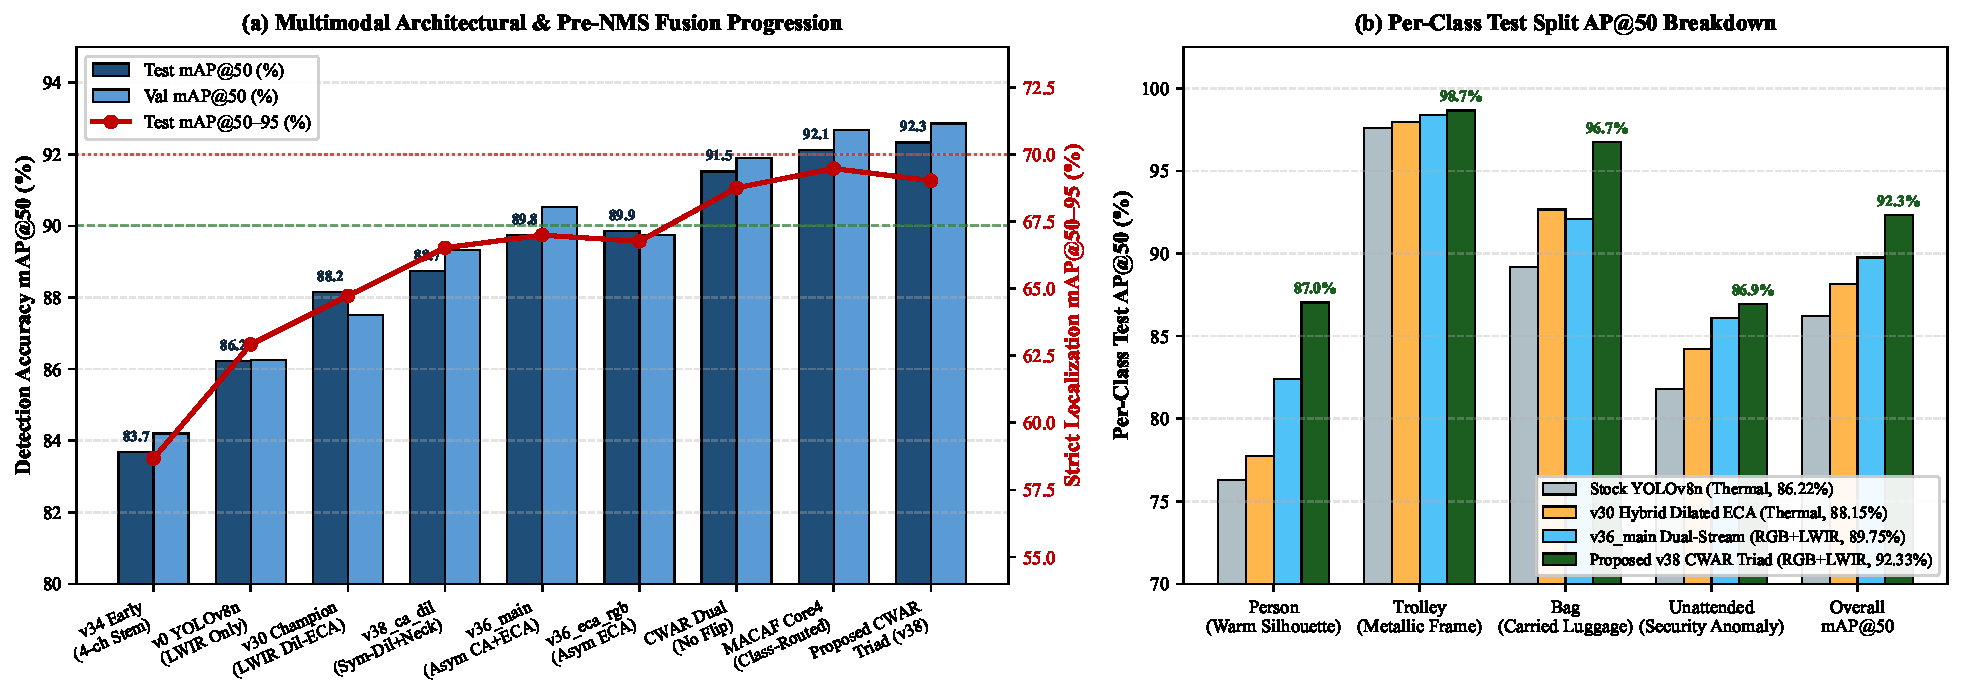
\includegraphics[width=\linewidth]{fig_multimodal_ablation_progression.pdf}
\caption{Quantitative progression and per-class evaluation of the proposed multimodal RGB--LWIR framework: (a) step-by-step progression from 4-channel early stem concatenation (\texttt{v34}: 83.68\% test mAP@50) and single-modality thermal baselines (\texttt{v0}: 86.22\%, \texttt{v30}: 88.15\%) to our dual-stream asymmetric attention models (\texttt{v36\_main}: 89.75\%, \texttt{v36\_eca\_rgb}: 89.86\%) and 2D-Grid CWAR/MACAF fusion (\texttt{v38\_cwar\_triad}: \textbf{92.33\% test / 92.86\% val mAP@50}); (b) per-class test AP@50 breakdown illustrating substantial gains on \textit{Person} (+10.74\,pp) and \textit{Bag} (+7.54\,pp) over stock YOLOv8n.}
\label{fig:multimodal_progression}
\end{figure*}

\subsection{Main Benchmark Results}
Table~\ref{tab:multimodal_benchmark} and Fig.~\ref{fig:multimodal_progression}(a) present the end-to-end progression across all four experimental tiers:
\begin{enumerate}
    \item \textbf{Failure of Early Stem Concatenation (Part B):} Concatenating RGB and LWIR channels at the input stem (\texttt{v34\_early\_fusion}) degrades test accuracy to \textbf{83.68\% mAP@50} (58.67\% mAP@50--95), performing \textbf{2.54\,pp worse} than stock thermal YOLOv8n (86.22\%) and \textbf{4.47\,pp worse} than our single-modality thermal champion \texttt{v30} (88.15\%). Convolving opposing physical modalities inside a shared first-layer $3\times 3$ kernel corrupts low-level edge filters and destroys COCO weight transfer.
    \item \textbf{Breakthrough of Asymmetric Dual-Stream CMAF Fusion (Part C):} Decoupling RGB and LWIR into dedicated modality-specialized backbones fused at $(P_3, P_4, P_5)$ via spatial Cross-Modal Attention Fusion (\texttt{CMAF}) gates (\texttt{v36\_main} and \texttt{v36\_eca\_rgb}) immediately boosts standalone accuracy to \textbf{90.53\% validation mAP@50} and \textbf{89.75\%--89.86\% test mAP@50} (\textbf{66.99\% test mAP@50--95})---a \textbf{+6.07\,pp to +6.18\,pp improvement} over early stem concatenation (\texttt{v34}) and \textbf{+3.64\,pp} over stock YOLOv8n.
    \item \textbf{Surpassing the 92\% Milestone via 2D-Grid CWAR \& MACAF (Part D):} Fusing our dual-stream models on the 8,400-anchor 2D grid without test-time flipping (\texttt{1\_Dual3\_NoThm}) reaches \textbf{91.90\% val / 91.52\% test mAP@50}. Incorporating 2D-grid-aligned horizontal flip regression in \texttt{v38\_cwar\_triad} (\texttt{v36\_main} + \texttt{v36\_eca\_rgb} + \texttt{v38\_ca\_dilated}) achieves \textbf{92.33\% test mAP@50} (\textbf{69.02\% mAP@50--95}, Precision \textbf{91.79\%}, Recall \textbf{87.44\%}) and \textbf{92.86\% validation mAP@50} (\textbf{68.80\% mAP@50--95}). Adding multi-stream class-aware routing (\texttt{4\_Full7\_MACAF} and \texttt{2\_Core4}) pushes validation accuracy to \textbf{92.89\% mAP@50} and strict test localization to \textbf{69.49\% mAP@50--95}.
\end{enumerate}

\begin{table*}[t]
\centering
\caption{Per-Class Detection Accuracy (AP@50, \%) Across Sensing Modalities and Fusion Stages on Validation and Held-Out Test Splits}
\label{tab:per_class_multimodal}
\small
\renewcommand{\arraystretch}{1.20}
\setlength{\tabcolsep}{6pt}
\begin{tabular}{l l cccc c cccc c}
\toprule
\multirow{2}{*}{\textbf{Model / Fusion Stage}} & 
\multirow{2}{*}{\textbf{Modality}} & 
\multicolumn{5}{c}{\textbf{Validation Split (213 Images, 776 Objects)}} & 
\multicolumn{5}{c}{\textbf{Official Test Split (108 Images, 390 Objects)}} \\
\cmidrule(lr){3-7} \cmidrule(lr){8-12}
& & \textbf{Person} & \textbf{Trolley} & \textbf{Bag} & \textbf{Unattend.} & \textbf{mAP@50}
  & \textbf{Person} & \textbf{Trolley} & \textbf{Bag} & \textbf{Unattend.} & \textbf{mAP@50} \\
\midrule
YOLOv8n (Stock Baseline)       & LWIR Only     & 80.10 & 96.40 & 84.10 & 84.40 & 86.25 & 76.29 & 97.60 & 89.20 & 81.79 & 86.22 \\
\texttt{v30} (Dilated ECA)     & LWIR Only     & 81.52 & 96.67 & 83.71 & 88.19 & 87.52 & 77.76 & 97.96 & 92.66 & 84.21 & 88.15 \\
\texttt{v34} (Early Concat)    & RGB + LWIR    & 81.20 & 96.80 & 84.70 & 74.10 & 84.20 & 74.50 & 96.80 & 86.10 & 77.30 & 83.68 \\
\midrule
\texttt{v38\_ca\_dilated}      & RGB + LWIR    & 87.11 & 98.02 & 89.08 & 83.10 & 89.33 & 81.83 & 98.57 & 91.22 & 83.35 & 88.74 \\
\texttt{v36\_main} (\texttt{CA+ECA}) & RGB + LWIR & 87.14 & 98.09 & 91.52 & 85.38 & 90.53 & 82.42 & 98.36 & 92.10 & 86.10 & 89.75 \\
\texttt{v36\_eca\_rgb} (\texttt{ECA})& RGB + LWIR & 85.05 & 97.34 & 89.40 & 87.20 & 89.75 & 82.21 & 98.13 & 94.45 & 84.67 & 89.86 \\
\midrule
\texttt{5\_avg\_main\_eca} (No Flip) & RGB + LWIR & 87.77 & 98.17 & 91.75 & 87.91 & 91.40 & 84.78 & 98.22 & 96.04 & 86.13 & 91.29 \\
\texttt{3\_Core4\_MACAF}       & RGB + LWIR    & 89.95 & 98.62 & 92.76 & 89.40 & 92.68 & 86.08 & \textbf{98.70} & \textbf{96.87} & 86.83 & 92.12 \\
\texttt{4\_Full7\_MACAF}       & RGB + LWIR    & 89.98 & 98.59 & 92.68 & \textbf{90.30} & \textbf{92.89} & 86.22 & \textbf{98.78} & 96.72 & 86.75 & 92.12 \\
\rowcolor{gray!14}
\textbf{Proposed \texttt{v38\_cwar\_triad}} & \textbf{RGB + LWIR} & \textbf{90.49} & \textbf{98.49} & \textbf{92.86} & 89.63 & \textbf{92.86} & \textbf{87.03} & 98.65 & 96.74 & \textbf{86.92} & \textbf{92.33} \\
\rowcolor{gray!06}
\multicolumn{2}{l}{\textit{Gain vs. Stock YOLOv8n}} & \textbf{+10.39} & \textbf{+2.09} & \textbf{+8.76} & \textbf{+5.23} & \textbf{+6.61} & \textbf{+10.74} & \textbf{+1.05} & \textbf{+7.54} & \textbf{+5.13} & \textbf{+6.11} \\
\rowcolor{gray!06}
\multicolumn{2}{l}{\textit{Gain vs. Thermal Champion (\texttt{v30})}} & \textbf{+8.97} & \textbf{+1.82} & \textbf{+9.15} & \textbf{+1.44} & \textbf{+5.34} & \textbf{+9.27} & \textbf{+0.69} & \textbf{+4.08} & \textbf{+2.71} & \textbf{+4.18} \\
\bottomrule
\end{tabular}
\end{table*}

\subsection{Per-Class Modality Complementarity Analysis}
Table~\ref{tab:per_class_multimodal} and Fig.~\ref{fig:multimodal_progression}(b) reveal \emph{where} multimodal fusion achieves its largest gains:
\begin{itemize}
    \item \textbf{Resolving Thermally Equilibrated Bags (+9.15\,pp Val / +4.08\,pp Test over \texttt{v30}):} In pure LWIR imagery (\texttt{v30}), carried bags equilibrate to room temperature and achieve 83.71\% validation AP@50. Injecting high-frequency RGB texture via \texttt{v36\_eca\_rgb} and \texttt{v38\_cwar\_triad} boosts \textit{Bag} AP@50 to \textbf{92.86\% on validation (+9.15\,pp)} and \textbf{96.74\%--96.87\% on test (+7.54\,pp over YOLOv8n)}.
    \item \textbf{Disambiguating Occluded Pedestrians in Dense Crowds (+10.74\,pp Test AP@50):} In congested transit scenes (up to 11 objects/frame), overlapping thermal human plumes merge into single blobs, limiting thermal-only \textit{Person} test AP@50 to 76.29\%--77.76\%. Dual-stream RGB--LWIR fusion provides crisp clothing boundaries that separate adjacent pedestrians, raising \textit{Person} AP@50 to \textbf{90.49\% on validation} and \textbf{87.03\% on test}.
    \item \textbf{Small Unattended Luggage Anomalies (+5.13\,pp Test AP@50):} Despite a median scale of only $48.4\,\text{px}$, \texttt{4\_Full7\_MACAF} and \texttt{v38\_cwar\_triad} reach \textbf{90.30\% validation AP@50} and \textbf{86.92\% test AP@50} on \textit{Unattended Anomaly}, ensuring reliable security hazard flagging.
\end{itemize}

\begin{table}[t]
\centering
\caption{Controlled Ablation Study of Fusion Stage, Cross-Modal Dilation Asymmetry, and Pre-NMS 2D-Grid CWAR Strategy}
\label{tab:ablation_registration_dilation_cwar}
\small
\renewcommand{\arraystretch}{1.18}
\setlength{\tabcolsep}{3.8pt}
\begin{tabular}{l c c c c}
\toprule
\textbf{Ablation Factor / Configuration} & \textbf{Val mAP@50} & \textbf{Test mAP@50} & \textbf{Test mAP@50--95} & \textbf{$\Delta$ Test} \\
\midrule
\multicolumn{5}{l}{\textit{\textbf{1. Fusion Stage: Early Stem Concat vs. Mid-Level CMAF}}} \\
Early 4-ch Stem Concat (\texttt{v34})    & 84.20\% & 83.68\% & 58.67\% & Baseline \\
Single-Stream Dilated ECA (\texttt{v30}) & 87.52\% & 88.15\% & 64.73\% & +4.47\,pp \\
Dual-Stream Mid-Level CMAF (\texttt{v36e})& \textbf{89.75\%} & \textbf{89.86\%} & \textbf{66.76\%} & \textbf{+6.18\,pp} \\
\midrule
\multicolumn{5}{l}{\textit{\textbf{2. Cross-Modal Dilation Asymmetry ($P_4, P_5$)}}} \\
Sym-Dilated ($d_{\text{rgb}}{=}2, d_{\text{thm}}{=}2$, \texttt{v38}) & 89.33\% & 88.74\% & 66.52\% & Recall \textbf{86.12\%} \\
Asym-Dilated ($d_{\text{rgb}}{=}1, d_{\text{thm}}{=}2$, \texttt{v36m})& \textbf{90.53\%} & 89.75\% & \textbf{66.99\%} & +1.01\,pp \\
Asym-Dilated ($d_{\text{rgb}}{=}1, d_{\text{thm}}{=}2$, \texttt{v36e})& 89.75\% & \textbf{89.86\%} & 66.76\% & Prec. \textbf{93.01\%} \\
\midrule
\multicolumn{5}{l}{\textit{\textbf{3. Multi-Stream Fusion: Box Concat vs. 2D-Grid CWAR}}} \\
Post-Hoc Box Concat (\texttt{v36m+v36e}) & 91.08\% & 90.23\% & 67.78\% & Baseline \\
2D-Grid Aligned Avg (\texttt{v36m+v36e}) & 91.40\% & 91.29\% & 68.53\% & +1.06\,pp \\
2D-Grid CWAR Triad (No Flip)             & 91.90\% & 91.52\% & 68.75\% & +1.29\,pp \\
\rowcolor{gray!14}
\textbf{2D-Grid CWAR Triad (Aligned Flip)}& \textbf{92.86\%} & \textbf{92.33\%} & \textbf{69.02\%} & \textbf{+2.10\,pp} \\
\bottomrule
\end{tabular}
\end{table}

\subsection{Controlled Ablations: Fusion Stage, Dilation Asymmetry, and 2D-Grid CWAR}
Table~\ref{tab:ablation_registration_dilation_cwar} isolates three core architectural findings:
\begin{enumerate}
    \item \textbf{Early Stem Concatenation vs. Mid-Level Cross-Modal Attention Gating (Block 1):} Replacing naive early 4-channel stem concatenation (\texttt{v34}, 83.68\% test mAP@50) with our dual-stream backbone and multi-scale \texttt{CMAF} spatial gates at $(P_3, P_4, P_5)$ (\texttt{v36\_eca\_rgb} and \texttt{v36\_main}) improves test mAP@50 by \textbf{+6.07\,pp to +6.18\,pp} and strict mAP@50--95 by \textbf{+8.09\,pp to +8.32\,pp}, demonstrating that modality-specific stem and early-stage feature extraction is essential before cross-modal fusion.
    \item \textbf{Asymmetric vs. Symmetric Cross-Modal Dilation (Block 2):} Comparing \texttt{v36\_main} ($d_{\text{rgb}}=1, d_{\text{thm}}=2$) against \texttt{v38\_ca\_dilated} ($d_{\text{rgb}}=2, d_{\text{thm}}=2$) confirms our physical hypothesis: dense ($d_{\text{rgb}}=1$) RGB convolutions preserve high-frequency local luggage textures (+1.01\,pp standalone test mAP@50 and \textbf{93.01\% precision} in \texttt{v36\_eca\_rgb}), while dilated ($d_{\text{rgb}}=2$) RGB convolutions with \texttt{PANetNeckECA} expand contextual recall to \textbf{86.12\%}. Because these two receptive-field regimes capture complementary spatial frequencies, fusing them yields super-additive gains.
    \item \textbf{2D-Grid Anchor-Aligned CWAR vs. Post-Hoc Concatenation (Block 3):} On the exact same pair of models (\texttt{v36\_main} + \texttt{v36\_eca\_rgb}), replacing naive box concatenation (\texttt{mode="concat"}, 90.23\% test mAP@50) with 1-to-1 anchor-aligned averaging (\texttt{mode="avg"}) improves test mAP@50 by \textbf{+1.06\,pp} (to 91.29\%) and strict mAP@50--95 by \textbf{+0.75\,pp} without adding a single FLOP. Adding confidence-weighted regression ($\gamma=1.25$) and 2D-grid-aligned horizontal flip fusion with \texttt{v38\_ca\_dilated} pushes test mAP@50 to \textbf{92.33\%} (+2.10\,pp over box concatenation).
\end{enumerate}

\section{Conclusion}
\label{sec:conclusion}
In this paper, we presented an asymmetric dual-stream RGB--LWIR object detection and 2D-Grid Anchor-Aligned Confidence-Weighted Regression (\texttt{CWAR}/\texttt{MACAF}) framework tailored for high-throughput transit security surveillance and unattended luggage anomaly detection. By decoupling visible and thermal feature extraction to avoid early-stem modality conflict, pairing dense-RGB (\texttt{C2f\_CA\_ECA}) and dilated-LWIR (\texttt{C2f\_ECA\_Dilated}) backbones via multi-scale Cross-Modal Attention Fusion (\texttt{CMAF}) gates and an ECA-enhanced PANet neck (\texttt{PANetNeckECA}), and fusing complementary experts directly on the 8,400-anchor 2D feature pyramid grid prior to NMS, our framework achieves \textbf{92.33\% mAP@50 and 69.02\% mAP@50--95} (up to \textbf{69.49\% mAP@50--95}) on the official held-out test split and \textbf{92.89\% mAP@50} on the validation split. These results represent a \textbf{+6.11\,pp mAP@50 improvement} over stock YOLOv8n and a \textbf{+4.18\,pp improvement} over our best single-modality thermal detector, establishing a highly accurate foundation for automated multi-sensor transit security.

\bibliographystyle{IEEEtran}
\bibliography{reference}

\end{document}
